\section{Results for Curriculum Reinforcement Learning} \label{sec: Results - Curriculum Reinforcement Learning}

In this final results section, we demonstrate the role of Curriculum Learning in enhancing the RL agent’s training process. By gradually increasing the complexity of the environment, we show how CL contributes to improved learning efficiency and overall performance. Obtained results are described in the following fashion:
First subsection describes a setting of a baseline results to verify the possible improvements that can be achieved with CL. Second and third subsections provide an understanding on the CL parameters selection. Fourth subsection describes the obtained results to create an overview of having CL enhancement, while the fifth subsection provides a comparison of the best achieved systems to the baseline. 

\subsection{Setting up a baseline}

Before proceeding with the analysis, it is essential to establish baseline results for the continuous RL PPO method, without enhancements from Curriculum Learning. This provides a point of reference to assess how much CL can improve performance. For this we have conducted tests using the system parameters presented in the Table~\ref{tab:hyperparameters} and~\ref{tab:env_params} for systems with 1 to 3 links. For each system, 10 distinct simulation cases were executed to account for variability in control due to different initial conditions. The baseline is determined by measuring the training timesteps required for success, focusing primarily on the mean and median values, which serve as the key performance indicators. Additionally, the minimum and maximum values provide insight into the range of results across cases. These metrics allow us to assess the general performance of PPO in continuous action space. Table~\ref{tab: baseline statistics for PPO in continuous action space} summarizes the results for the RL training using the PPO algorithm in continuous action space. The results are presented for systems with 1, 2, and 3 links.

\begin{table}[ht]
	\centering
	\caption{Baseline results of using PPO algorithm in continuous action space for 1 to 3 link pendulum systems}
	\begin{tabular}{@{}lccccc@{}}
		\toprule
		\textbf{System} & \textbf{Successful cases} & \textbf{Mean} & \textbf{Median} & \textbf{Minimum} & \textbf{Maximum} \\ \midrule
		\textit{1-link} & 10 & 26168 & 25600 & 24320 & 32000 \\
		\textit{2-link} & 7 & 48055 & 49152 & 38400 & 55296 \\
		\textit{3-link} & 5 & 278937 & 288768 & 194560 & 319488 \\ \bottomrule
	\end{tabular}
	\label{tab: baseline statistics for PPO in continuous action space}
\end{table}

As indicated in Table~\ref{tab: baseline statistics for PPO in continuous action space}, the results show a clear progression in training time as the system complexity increases from 1-link to 3-link. The 1-link system requires the least number of timesteps on average to reach successful training, while the 3-link system exhibits significantly higher values, with a mean training time nearly 10 times longer than the 1-link system. This demonstrates that as the system complexity increases, the training duration grows substantially, making it harder for the PPO algorithm to converge quickly.

The primary goal of introducing CL enhancement is to accelerate the training process and potentially make the system more robust to various initial conditions. By progressively increasing the difficulty of the tasks during training, we aim to reduce the number of timesteps required for convergence. To further explore the impact of CL, the next step focuses on selecting the appropriate CL implementation parameters, dividing the research into well-defined steps. 

\subsection{Selection of a decay function}

To identify the most effective decay function for stabilizing the pendulum systems, we evaluated all previously introduced decay functions (described in Section~\ref{subsec: Curriculum learning implementation}) on a single pendulum system. Our goal was to determine which decay function led to the highest success rate in training the RL agent. We performed 150 simulation runs per decay function across 5 different initialization cases, each representing different system initial conditions, varying the control\todo{Reffering the "control" values is inconsistent as we have MSD parameters.} values vector \(\begin{bmatrix} 1 & n \end{bmatrix}\), where $n$ took values from the set \{2, 4, 6, 8, 10\}. Additionally, the decay steps $k$ ranged from 5000 to 10,000, with increments of 1000, to assess performance under different CL enhancement training time.

The control values represent the magnitude of assistance provided by the curriculum at each stage of training, while the decay steps govern how quickly the assistance diminishes. The system starts with significant assistance (higher values of $n$) and gradually transitions to full autonomy as the decay steps progress. This setup allows the RL agent to focus on stabilizing the pendulum with progressively less support as the training advances.

The results of these experiments are summarized in Figure~\ref{fig: decay types comparison}, which displays the number of successfully trained agents out of 150 for each decay function. The success of an agent was determined by its ability to stabilize the pendulum consistently across all test runs, meeting predefined performance thresholds.

\begin{figure}[h]
	\centering
	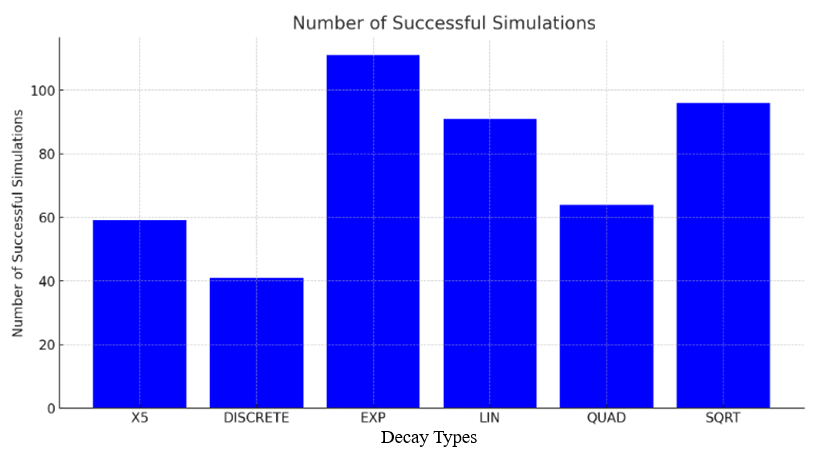
\includegraphics[width=12cm]{Figures/decay_types_results_comparison.png}
	\caption{Simulation results for decay function analysis. The bar plot represents the number of successfully trained agents out of 150 per decay function.}
	\label{fig: decay types comparison}
\end{figure}

As seen in the figure, the exponential decay function outperformed the other decay types, achieving a success rate of 74\%. This indicates that a faster initial reduction in assistance, followed by a gradual tapering off, is most conducive to training the agent for this particular task. The quadratic and square root decay functions also performed reasonably well but did not achieve the same level of consistency. The linear decay function, which reduces assistance at a constant rate, yielded lower success rate, suggesting that a more aggressive reduction in assistance is needed early in the training process to encourage the agent to adapt to the system’s dynamics more efficiently.

Based on these results, we selected the exponential decay function for later experiments, as it provided the most reliable improvement in training success across the tested scenarios. This decision allows us to proceed with further analysis using an exponential decay function.

\subsection{Selection of a decay factor}

To select the most suitable decay factor for training efficiency, we conducted an extensive analysis using a double pendulum system. The control values vector was set as \(\begin{bmatrix} 1 & n & n \end{bmatrix}\), where \(n = 1, 2, \ldots, 10\). For each unique combination of control values, decay steps, and decay factors, we ran 10 cases, with each case corresponding to different initial conditions. This ensured robustness and reliability in the results. In total, 5600 unique test cases were analyzed, covering a comprehensive range of conditions.

We investigated four decay factors: 0.005, 0.01, 0.05, and 0.5. The key metric used to evaluate the performance of each decay factor was the number of training timesteps required to reach successful stabilization. The shorter the training time, the more efficient the learning process, making the reduction in timesteps a critical indicator of the optimal decay factor.

\begin{figure}[h] 
	\centering 
	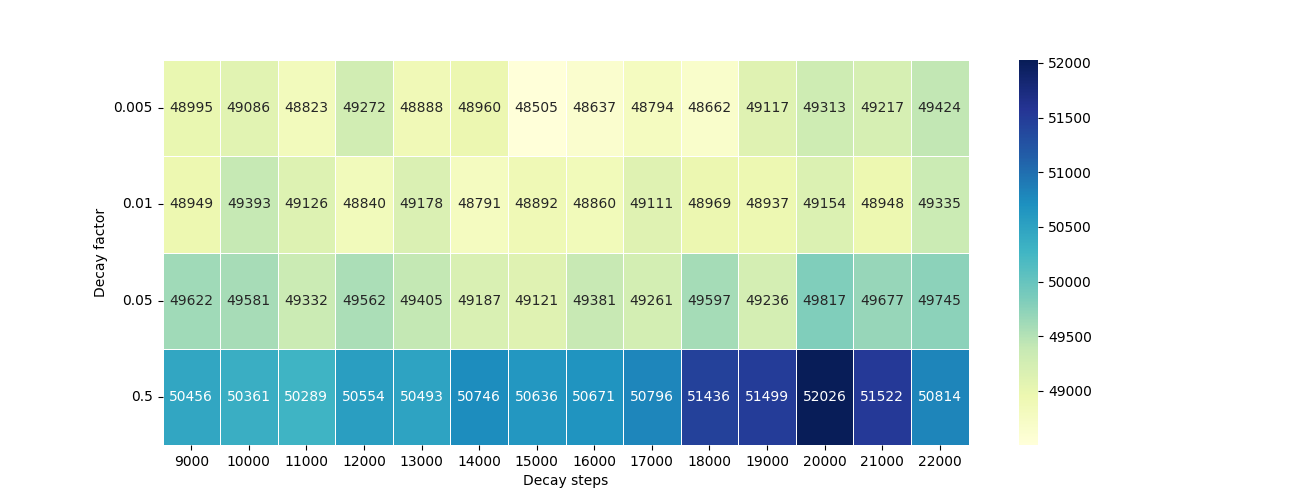
\includegraphics[width=15cm]{Figures/MaxSuccessfulTestsTimesteps_heatmap.png} 
	\caption{Heatmap showing the impact of different decay factors on the number of successful tests and timesteps. The decay factor 0.005 consistently performs best in terms of minimizing timesteps.} 
	\label{fig: decay factors comparison}
\end{figure}

As illustrated in Figure~\ref{fig: decay factors comparison}, the decay factor 0.005 consistently resulted in the lowest training timesteps across all combinations of control values and decay steps. This indicates that the system converged faster and more efficiently with this decay factor compared to the others. The findings suggest that a slower and more gradual reduction of assistance, as dictated by the decay factor 0.005, enables the RL agent to adapt more effectively, making it the optimal choice for this training setup. 

By contrast, larger decay factors, such as 0.05 and 0.5, showed longer training times, implying that the more rapid reduction in assistance restricted the agent's ability to efficiently learn the system's dynamics. Thus, the decay factor 0.005 was selected to proceed with to ensure more efficient learning with minimized training time.

\subsection{CL enhancement: overview} 

Having selected the appropriate decay function and decay factor for our task, we proceeded with simulations to explore the remaining Curriculum Learning (CL) parameters: control values and decay steps. The system was tested under different combinations of these parameters in all three environments (1-link, 2-link, and 3-link systems).
Each environment was evaluated using a specific control value scheme and a corresponding range of decay steps:
\begin{itemize}
	\item \textbf{1-link environment:} control values scheme as \(\begin{bmatrix} 1 & n \end{bmatrix}\), where at first $n$ varied from 0.1 to 1 (step size of 0.1) with decay steps varied from 1000 to 10000, and at second $n$ is varied from 1 to 12 (step size of 1) with decay steps varied from 4000 to 12000.
	\item \textbf{2-link environment:} control values scheme as \(\begin{bmatrix} 1 & 4n & n \end{bmatrix}\), where $n$ varied from 1 to 10 (step size of 1) and decay steps varied from 9000 to 22000.
	\item \textbf{3-link environment:} control values scheme as \(\begin{bmatrix} 1 & 4n & 2n & n \end{bmatrix}\), where $n$ varied from 1 to 10 (step size of 1) and decay steps varied from 30000 to 50000.
\end{itemize}

Our assumptions were that as the system complexity increases (more links), greater spring-damper influence would be required to stabilize the system, particularly for the first link, which bears the weight of the subsequent links. Based on preliminary experiments, it was determined that a strong cart restriction was unnecessary, so a fixed control value of 1 was used for cart translational movement in all simulations. To explain the selection of decay steps per system one factor is important, which is a system training time without CL. Since more training time is required as the system being more complex - it is needed to have higher values of decay steps to go through the training period with CL enhancement.

The evaluation of results was performed across cases within each unique combination of control values and decay steps. Simulation parameters for all 3 systems are taken from the Table~\ref{tab:env_params}. To show the obtained results a specific heatmap is provided. Each heatmap cell is a mean value of the training time of 10 cases under specific combination of control values and decay steps. Each case out of 10 represents a pendulum system under different initial conditions, so that training 10/10 cases is considered as successful and the robustness of the proposed training framework is evaluated. The results are shown in the Figure~\ref{fig: CL heatmaps}: (a) and (b) provide the 1-link system resulted heatmaps, while (c) and (d) represent the results for 2- and 3- link systems.

\begin{figure}[h!]
	\centering
	\begin{subfigure}[t]{0.48\textwidth}
		\centering
		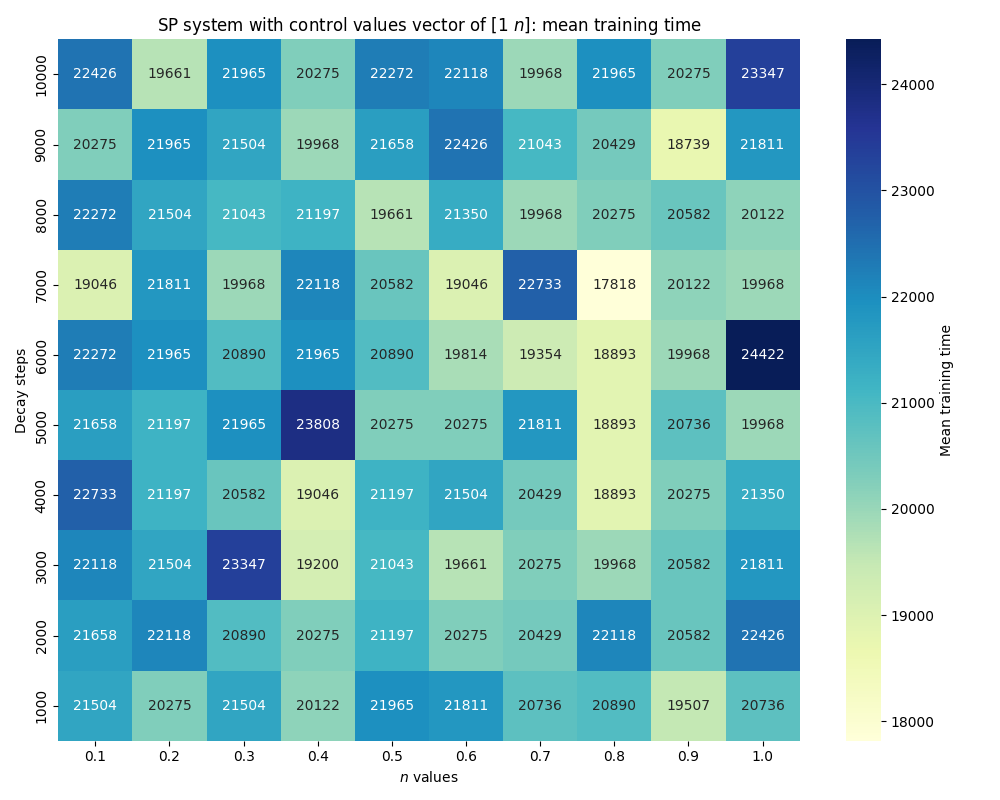
\includegraphics[width=\textwidth]{Figures/SP_cv_01_to_1.png}
		\caption{1-link: control values varied from 0.1 to 1, decay steps range from 1000 to 10000}
	\end{subfigure}
	\begin{subfigure}[t]{0.48\textwidth}
		\centering
		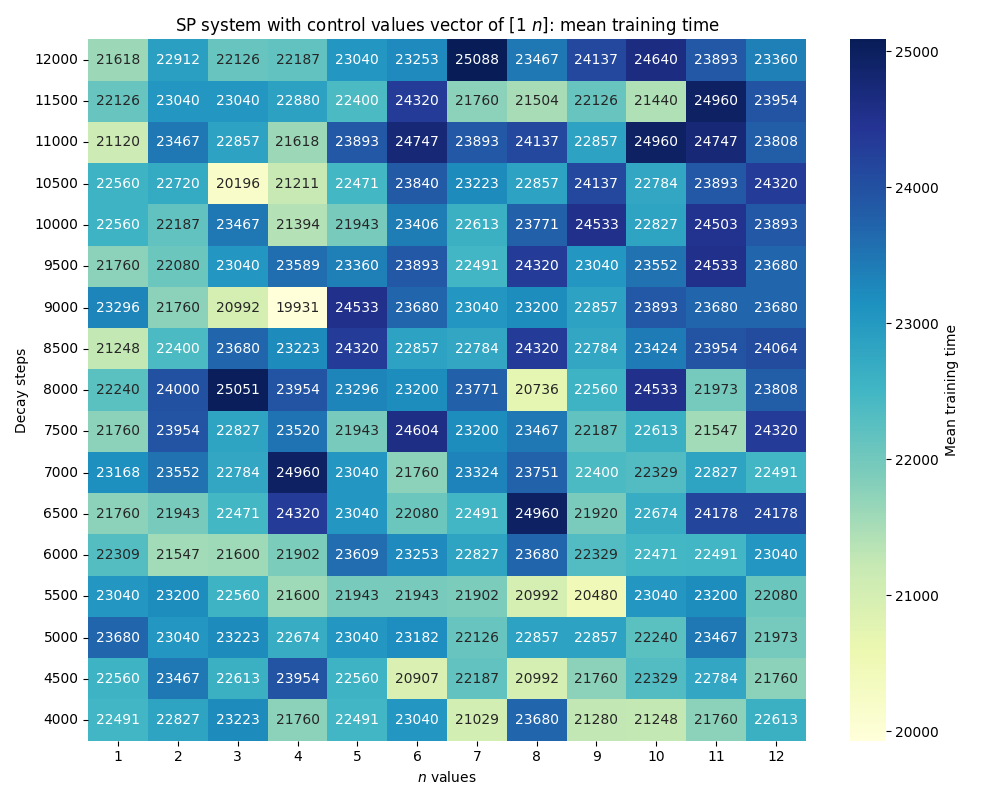
\includegraphics[width=\textwidth]{Figures/SP_cv_1_to_12.png}
		\caption{1-link: control values varied from 1 to 12, decay steps range from 4000 to 12000}
	\end{subfigure}
	\begin{subfigure}[t]{0.48\textwidth}
		\centering
		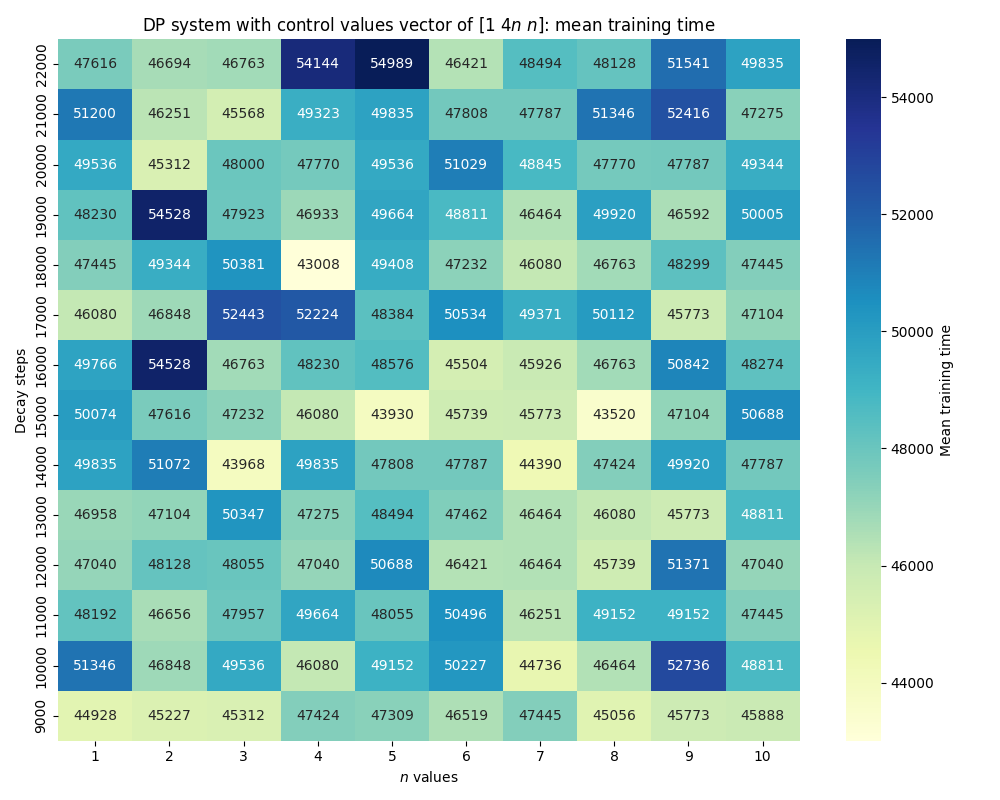
\includegraphics[width=\textwidth]{Figures/DP_1_4n_n_heatmap_mean.png}
		\caption{2-link: $n$ value varied from 1 to 10, decay steps range from 9000 to 22000}
	\end{subfigure}
	\begin{subfigure}[t]{0.48\textwidth}
		\centering
		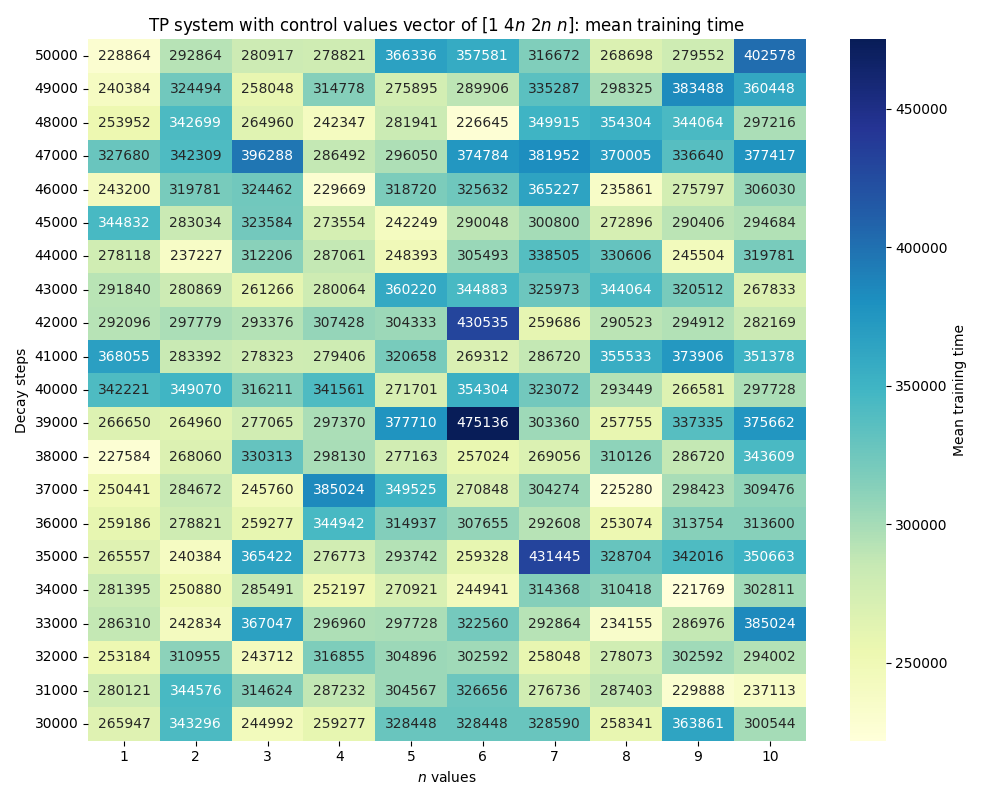
\includegraphics[width=\textwidth]{Figures/TP_1_4n_2n_n_heatmap_mean.png}
		\caption{3-link: $n$ value varied from 1 to 10, decay steps range from 30000 to 50000}
	\end{subfigure}
	
	\caption{Heatmaps with mean system training time for 1-link (a), (b), for 2-link (c) and 3-link (d) systems under various control values and decay steps}
	\label{fig: CL heatmaps}
\end{figure}

For the 1-link system (Figures~\ref{fig: CL heatmaps} (a) and (b)), the mean training times ranged between 18,000 and 25,000 timesteps. The results demonstrate that lower values of \(n\) (i.e., less restriction on the pendulum) led to faster training times. Increasing \(n\) significantly raised the mean training time, indicating that greater restriction of the pendulum caused a slowdown in learning. Higher restrictions resulted in performance close to the baseline without CL, suggesting that over-constraining the system negatively impacts the RL agent's learning efficiency.

In the 2-link system (Figure~\ref{fig: CL heatmaps} (c)), the results are more variable. While some parameter combinations resulted in relatively low mean training times around 43,000 timesteps, no consistent pattern emerged for the decay steps and control values. Despite this, we observed an improvement compared to baseline results without CL, indicating that CL can still be effective, but only under certain conditions. However, the lack of a clear pattern suggests that tuning these parameters requires trial and error, and the improvements are not as significant as initially expected.

The 3-link system (Figure~\ref{fig: CL heatmaps} (d)) yielded the most promising results, with nearly 50\% of the combinations showing faster training times compared to the baseline. The improvements seen were substantial but irregular -- like the 2-link system, there was no clear pattern in the best-performing parameter combinations. This indicates that while CL can indeed improve performance, the lack of systematic guidelines for selecting optimal parameters presents a challenge.

From this analysis, it can be concluded that Curriculum Learning can indeed improve RL training, but its effectiveness is highly dependent on specific parameter settings, such as decay steps and control values. These parameters vary significantly depending on the system's complexity, and selecting the optimal combination may require extensive trial and error. While the results are encouraging for certain cases, especially in the 3-link system, the inconsistent improvements across different parameter settings highlight the need to develop more systematic methods for selecting CL parameters.

\subsection{CL enhancement: evaluation of the best performing schemes}

From the results obtained in the previous section, it is possible to compare the best-achieved results to the established baseline without CL for our task. To select the best performing scheme, two metrics were taken into account: the number of successful cases per cell and the mean training time. By combining these two criteria, the CL-enhanced system becomes both robust across cases and faster in terms of training time. The number of successful cases per cell is not shown on the heatmaps to avoid overloading the visual representation and is instead extracted directly from the results datasets. For the 1-link and 2-link systems, a successful case was defined as achieving 50 out of 50 successful tests. For the 3-link system, due to its higher complexity, the threshold for success was set at 70 out of 100 tests passed. The full description of the evaluation framework is provided in Section~\ref{subsec: Model evaluation}. The selected best performing schemes are shown in Table~\ref{tab: CL results}.

\begin{table}[ht]
	\centering
	\caption{CL enhancement: best control values schemes -- results for 1- to 3- link pendulum systems}
	\begin{tabular}{@{}lccc@{}}
		\toprule
		\textbf{System} & \makecell{\textbf{Best performing}\\ \textbf{schemes}} & \makecell{\textbf{Successful}\\ \textbf{cases}} & \makecell{\textbf{Decay}\\ \textbf{steps}} \\ \midrule
		\textit{1-link} & \(\begin{bmatrix} 1 & 0.8 \end{bmatrix}\) & 10 & 7000 \\ \midrule
		\textit{2-link} & \(\begin{bmatrix} 1 & 20 & 5 \end{bmatrix}\) & 10 & 15000 \\ \midrule
		\textit{3-link} & \(\begin{bmatrix} 1 & 16 & 8 & 4 \end{bmatrix}\) & 10 & 30000 \\ \bottomrule
	\end{tabular}
	\label{tab: CL results}
\end{table}

All three systems achieved 10/10 successful cases, confirming their robustness. The assumption that higher decay steps are needed as system complexity increases is validated. Having established the best performing schemes, we compare them to the baseline using a candle plot, where the primary comparison factor is the mean training time. Results are shown in Figure~\ref{fig: CL results comparison}.

\begin{figure}[h!]
	\centering
	\begin{subfigure}[t]{0.48\textwidth}
		\centering
		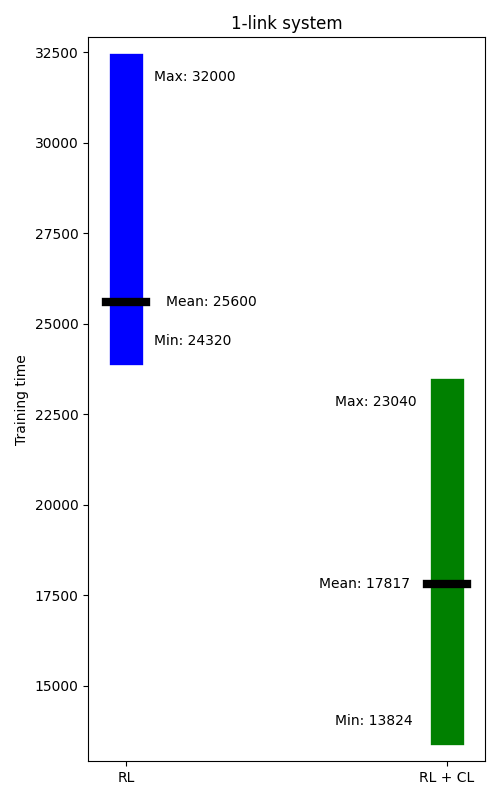
\includegraphics[width=\textwidth]{Figures/1_link_comparison.png}
		\caption{1-link. 30\% mean training time improvement for RL + CL}
	\end{subfigure}
	\begin{subfigure}[t]{0.48\textwidth}
		\centering
		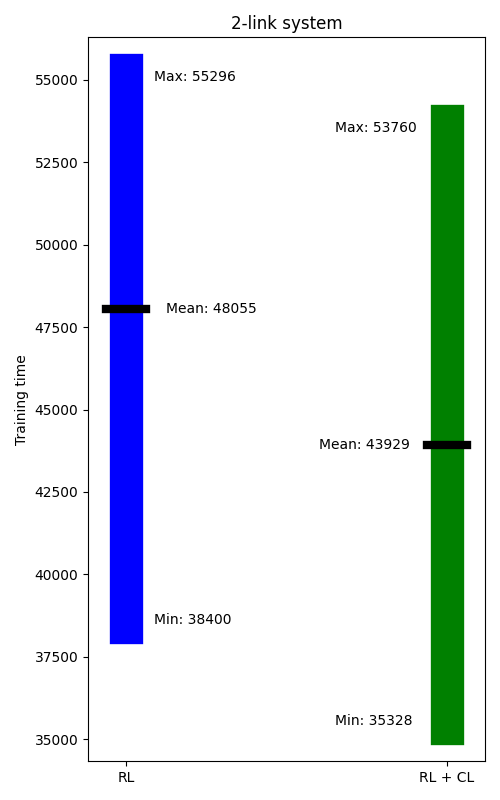
\includegraphics[width=\textwidth]{Figures/2_link_comparison.png}
		\caption{2-link. 10\% mean training time improvement for RL + CL}
	\end{subfigure}
	\begin{subfigure}[t]{0.48\textwidth}
		\centering
		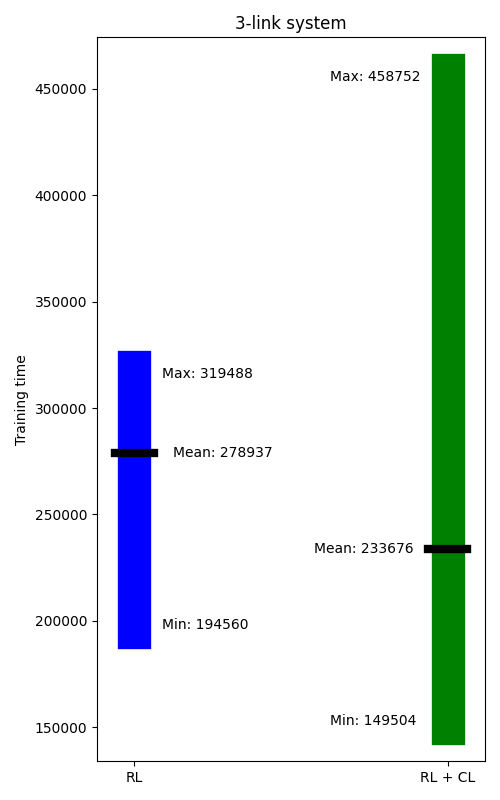
\includegraphics[width=\textwidth]{Figures/3_link_comparison.png}
		\caption{3-link. 17\% mean training time improvement for RL + CL}
	\end{subfigure}
	
	\caption{Training time comparison between RL and RL + CL approaches: 1-link (a), 2-link (b), 3-link (c).}
	\label{fig: CL results comparison}
\end{figure}

These results highlight the robustness of the implemented Curriculum Learning in reducing training times while maintaining high success rates, even as system complexity increases. To gain further insights into how the variations in control schemes and decay steps influenced the training times, we present a series of heatmaps in Figure~\ref{fig: percentage heatmaps for 1- to 3- link systems using CL} (a) to (f). The percentage change in both mean and median training times for each pendulum system is visualized, providing a clear depiction of the impact of CL enhancements across different cases.

\begin{figure}[h!]
	\centering
	\begin{subfigure}[t]{0.48\textwidth}
		\centering
		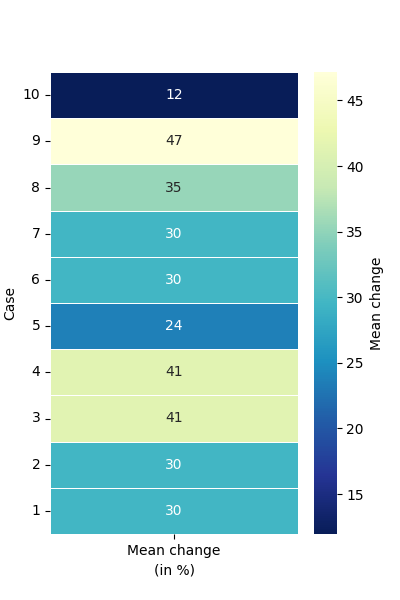
\includegraphics[width=\textwidth]{Figures/SP_mean_heatmap_percentage.png}
		\label{fig: SP_mean}
		\caption{}
	\end{subfigure}
	\hfill
	\begin{subfigure}[t]{0.48\textwidth}
		\centering
		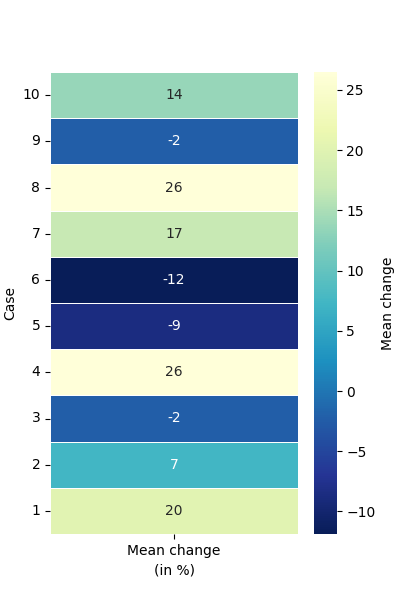
\includegraphics[width=\textwidth]{Figures/DP_mean_heatmap_percentage.png}
		\label{fig: DP_mean}
		\caption{}
	\end{subfigure}
	\hfill
	\begin{subfigure}[t]{0.48\textwidth}
		\centering
		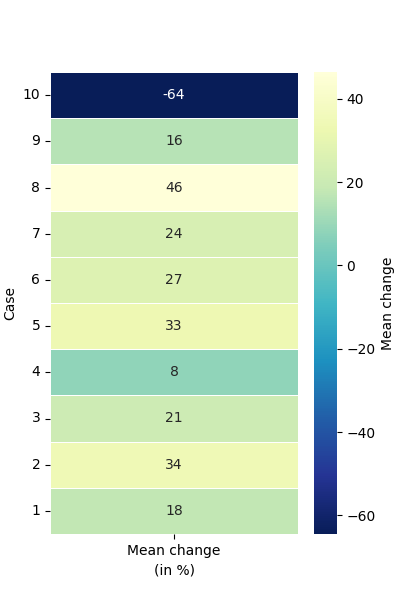
\includegraphics[width=\textwidth]{Figures/TP_mean_heatmap_percentage.png}
		\label{fig: TP_mean}
		\caption{}
	\end{subfigure}
	\hfill
	
	\caption{Mean training time change per cases for pendulum systems using CL enhancement: 1-link (a), 2-link (b), 3-link (c). Mean change per case is represented in \% and shows how does a training time of a case differs from the baseline mean. A positive change represents that the specific case is trained faster, while a negative change means that this case is worse than the baseline mean training time.}
	\label{fig: percentage heatmaps for 1- to 3- link systems using CL}
\end{figure}

The heatmaps demonstrate that across all systems, the implementation of CL resulted in significant improvements in training time for most cases. The 1-link system showed the greatest consistency in improvement, while the 2-link and 3-link systems demonstrated more variability, with some cases showing smaller improvements or even slower training times.

Overall, the results show that achieving the maximum number (10/10) of successfully trained cases is possible for each system, with a reduction in overall training time. However, the search for optimal CL parameters remains crucial, as no clear pattern emerges in the combination of control values and decay steps -- finding the best parameters is key to maximizing the benefits of CL. While our results show improvements, further fine-tuning of the parameters could lead to even faster training, especially in more complex systems.